\documentclass[a4paper,12pt]{article}

\usepackage[latin1,utf8]{inputenc}
\usepackage[portuges]{babel}
\usepackage{amsmath}
\usepackage{fancyhdr}
\usepackage{amssymb}
\usepackage{graphicx}
\usepackage{wrapfig}
\usepackage{picins}
\usepackage{physics}
\usepackage{blindtext}
\usepackage[a4paper,portrait]{geometry}  % Tipo de papel

\topmargin = 10pt                        % Margem superior: 20pt  
\textheight = 622pt                      % Altura do texto: 592pt

\begin{document}

%
% Inclusão de Imagens
%
%    \includegraphics[attr1=val1, attr2=val2, ..., attrn=valn]{imagename}
%
% Exemplos:
%    \includegraphics[width=\textwidth]{imagefile.pdf}
%    \includegraphics[width=5cm,height=5cm,keepaspectratio]{imagefile.pdf}
%    \includegraphics[width=5cm,height=5cm]{imagefile.pdf}
%

\begin{enumerate}
\item akakjas askjasas asashkas askaskas ashkashk askkjas  asjjaskljas asjsa asjjask askjas askljsakjas
 akakjas askjasas asashkas askaskas ashkashk askkjas  asjjaskljas asjsa asjjask askjas askljsakjas
 akakjas askjasas asashkas askaskas ashkashk askkjas  asjjaskljas asjsa asjjask askjas askljsakjas
Como segundo exemplo é apresentada uma imagem inserida à direita de
um bloco de texto.
\item
    \parpic(2in,1.5in)[r]{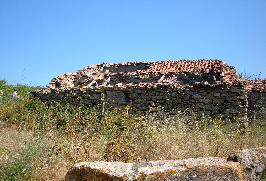
\includegraphics[width=2in]{dscf1683b_v1.jpg}}
    akakjas askjasas asashkas askaskas ashkashk askkjas  asjjaskljas asjsa asjjask askjas askljsakjas
    akakjas askjasas asashkas askaskas ashkashk askkjas  asjjaskljas asjsa asjjask askjas askljsakjas
   akakjas askjasas asashkas askaskas ashkashk askkjas  asjjaskljas asjsa asjjask askjas askljsakjas
 akakjas askjasas asashkas askaskas ashkashk askkjas  asjjaskljas asjsa asjjask askjas askljsakjas
   akakjas askjasas asashkas askaskas ashkashk askkjas  asjjaskljas asjsa asjjask askjas askljsakjas
 akakjas askjasas asashkas askaskas ashkashk askkjas  asjjaskljas asjsa asjjask askjas askljsakjas
   akakjas askjasas asashkas askaskas ashkashk askkjas  asjjaskljas asjsa asjjask askjas askljsakjas
\item akakjas askjasas asashkas askaskas ashkashk askkjas  asjjaskljas asjsa asjjask askjas askljsakjas
 akakjas askjasas asashkas askaskas ashkashk askkjas  asjjaskljas asjsa asjjask askjas askljsakjas
   akakjas askjasas asashkas askaskas ashkashk askkjas  asjjaskljas asjsa asjjask askjas askljsakjas
   akakjas askjasas asashkas askaskas ashkashk askkjas  asjjaskljas asjsa asjjask askjas askljsakjas
    \parpic(2in,1.5in)[l]{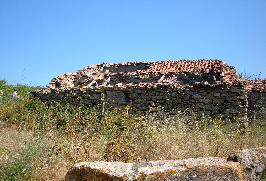
\includegraphics[width=2in]{dscf1683b_v1.jpg}}
   akakjas askjasas asashkas askaskas ashkashk askkjas  asjjaskljas asjsa asjjask askjas askljsakjas
   akakjas askjasas asashkas askaskas ashkashk askkjas  asjjaskljas asjsa asjjask askjas askljsakjas
 akakjas askjasas asashkas askaskas ashkashk askkjas  asjjaskljas asjsa asjjask askjas askljsakjas
   akakjas askjasas asashkas askaskas ashkashk askkjas  asjjaskljas asjsa asjjask askjas askljsakjas
 akakjas askjasas asashkas askaskas ashkashk askkjas  asjjaskljas asjsa asjjask askjas askljsakjas
   akakjas askjasas asashkas askaskas ashkashk askkjas  asjjaskljas asjsa asjjask askjas askljsakjas
\end{enumerate}

\break
   
Um condensador de placas paralelas tem uma área $A = 0.1\,$m$^2$ e uma distância
entre as placas $d = 3\,$mm. A meio, no seu interior, está uma placa de nylon de espessura
$s = 1$~mm. A constante dieléctrica relativa do nylon é de $\epsilon_r = 3.4$,
e suporta um campo eléctrico máximo de $14 \times 10^6$~V/m.

\begin{wrapfigure}[6]{l}{0.33\textwidth}
\centering
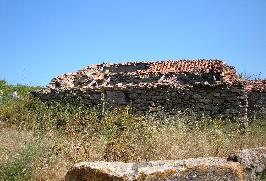
\includegraphics[width=0.3\textwidth, height=2cm, scale=1, angle=0]{dscf1683b_v1.png}
\end{wrapfigure}
A constante dieléctrica relativa do ar é de $\epsilon_r = 1.00059 \simeq 1$, e suporta
um campo eléctrico máximo de $3 \times 10^6$~V/m. Uma das armaduras tem uma carga
$Q = 1.5 \times 10^{-8}$~C (a outra tem uma carga --Q). Calcule, justificando:
   akakjas askjasas asashkas askaskas ashkashk askkjas  asjjaskljas asjsa asjjask askjas askljsakjas
 akakjas askjasas asashkas askaskas ashkashk askkjas  asjjaskljas asjsa asjjask askjas askljsakjas
   akakjas askjasas asashkas askaskas ashkashk askkjas  asjjaskljas asjsa asjjask askjas askljsakjas

\vskip 10mm
\centerline{\Large\bf Inclusão de imagem 'png'}
\par\vskip 5mm
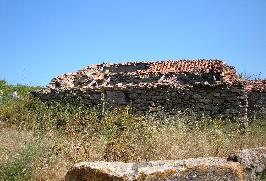
\includegraphics{dscf1683b_v1.png}

\break

\vskip 20mm
\centerline{\Large\bf Inclusão de imagem 'jpg'}
\par\vskip 5mm
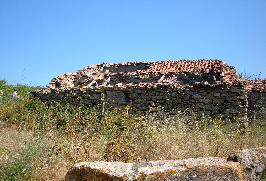
\includegraphics[width=5cm,height=5cm]{dscf1683b_v1.jpg}
\hskip 20mm
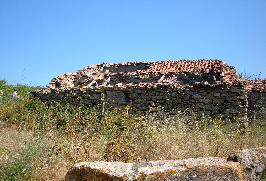
\includegraphics[width=5cm,height=5cm,keepaspectratio]{dscf1683b_v1.jpg}

\vskip 20mm
\centerline{\Large\bf Inclusão de imagem 'pdf'}
\par\vskip 5mm
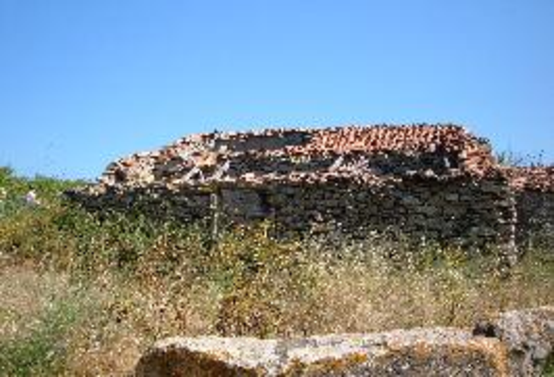
\includegraphics[width=3cm,height=3cm,keepaspectratio]{dscf1683b_v1.pdf}

\end{document}

